\section{Analyzing the Race-Honeypot}
\label{appendix:racehoneypot}
This part of the appendix will be used to present additional details about the race-honeypot that was found using \textsc{Amphicyon}. Especially, the traces of the transaction race are explained in detail. The \texttt{GIFT_CARD}-contract that is being analyzed here can be found on the Ethereum Blockchain at \cite{etherscan:giftcard}.

\subsection{The Honeypot Source Code}
As every honeypot, the \texttt{GIFT_CARD}-honeypot, whose source code is displayed in listing \ref{lst:honeypot:transactionrace}, contains an obvious "bug" making the victim interested in hacking the contract. In this case, the hash value restricting access to the "gift" can be overwritten when sending another 0.2 Ether to the \mintinline{solidity}{Put()}-function after it has already been set up.

\begin{listing}[H]
	\begin{minted}[
        linenos=true,
        firstnumber=1
    ]{solidity}
contract GIFT_CARD {
    function Put(bytes32 _hash, uint _unlockTime) public payable {
        if(!locked && msg.value > 200000000000000000)// 0.2 ETH {
            unlockTime = now+_unlockTime;
            hashPass = _hash;
        }
    }
    
    function Take(bytes _pass) external payable access(_pass) {
        if(hashPass == keccak256(_pass) && now>unlockTime && msg.sender==tx.origin) {
            msg.sender.transfer(this.balance);
        }
    }
    
    function Lock(bytes _pass) external payable access(_pass) {
        locked = true;
    }
    
    modifier access(bytes _pass) {
        if(hashPass == keccak256(_pass) && now>unlockTime && msg.sender==tx.origin)
            _;
    }
    
    bytes32 public hashPass;
    uint public unlockTime;
    bool public locked = false;
    
    function GetHash(bytes pass) public constant returns (bytes32) {return keccak256(pass);}
    
    function() public payable{}
}
    \end{minted}
	\caption{The \texttt{GIFT_CARD}-honeypot smart contract source code}
	\label{lst:appendix:giftcard}
\end{listing}

As a bait, during setup the \texttt{GIFT_CARD} had received 0.2 Ether using a \mintinline{solidity}{Put(0x..., 0)}-call.

As the first step of the attempt to hack the honeypot, the victim sent the 0.2 ether along with a call to \mintinline{solidity}{Put(0x..., 0)}. When starting the transaction for retrieval, another transaction was spawned attempting to retrieve the ether as well:

\subsection{Two conflicting transactions} At block height \texttt{5849419} two transactions were received by the contract: The first one having a hash starting with \texttt{0xe4e2d96}, that was started by the victim, and the second one with a hash of \texttt{0xb22467}, both calling \mintinline{solidity}{Take("65313763...")} with the same secret value to retrieve the "gift" from the contract.

While the average gas price of transactions in this block was \( 13.5 \textnormal{ Gwei} \)\footnote{\( \approxeq \frac{0.1081 \cdot 10^9}{7983695} \), which is the block reward divided by the gas used in the block \cite{etherscan:giftcard}}, both of those transactions had considerably higher gas prices:

To maximize profit, the miner chose to include transactions from the transaction pool starting with the one with the highest gas price: While transaction \texttt{0xb22467} had a gas price of \( 41 \textnormal{ Gwei} \), it was included as the 18th transaction of the block. \texttt{0xe4e2d96}s gas price was almost exactly \( 5 \) times higher at about \( 205 \textnormal{ Gwei} \), making it the highest gas price of this block and therefore the first transaction to be included by the miner. Because of this, the complete "gift" was sent to the creator of the second transaction, and not to the address of the victim.

\subsection{Interpretation}
The only way this could have worked is that the person behind address \texttt{0xbd7d} had been watching the incoming transactions in the transaction pool for a transaction calling \mintinline{solidity}{Take()} on the honeypot contract. Once the transaction of the victim was received which contained the plain-text of the hash stored in the contract an identical \mintinline{solidity}{Take()}-transaction was issued with a higher gas price, hoping for this transaction to be included first.

A strong indicator that the transaction with the higher gas price was issued by the same person that created the honeypot can be seen in the cash flow graph, that is displayed in figure \ref{figure:appendix:giftcard:transactiongraph}: The address starting with \texttt{0xbd7d} that withdrew the bait along with the yielded ether had indirectly sent the Ether to the address starting with \texttt{0xff17} that created the honeypot contract.

\vspace{1em}
\begin{minipage}{\linewidth}
	\centering
	\includegraphics[width=14cm]{img/giftcard/cashflowgraph.pdf}
	\captionof{figure}[Cash flow of GIFT_CARD]{Cash flow of the \texttt{GIFT_CARD}-honeypot. Contracts are rectangles, user addresses are drawn ovals.}
	\label{figure:appendix:giftcard:transactiongraph}
\end{minipage}

\subsection{Amphicyon Analysis Result}
This smart contract was only detected by \textsc{Amphicyon} during the mass-analysis of the latest 8000 smart contracts on Etherscan. While of course no underhanded solidity pattern could be detected, the contract was flagged due to different reasons, as can be seen in figure \ref{figure:appendix:giftcard:amphicyon}.

Next to standard, but not very strong signs of a honeypot like an uppercase name or the ability to send ether, some other typical honeypot coding pattern could be found: A initialization phase was implemented, and many functions were surrounded with an \mintinline{solidity}{if}-clause making the function fail silently if the condition evaluated to be wrong. Especially the later ones increased the honeypot probability ratio and therefore made \textsc{Amphicyon} flag the contract.

\vspace{1em}
\begin{minipage}{\linewidth}
	\centering
	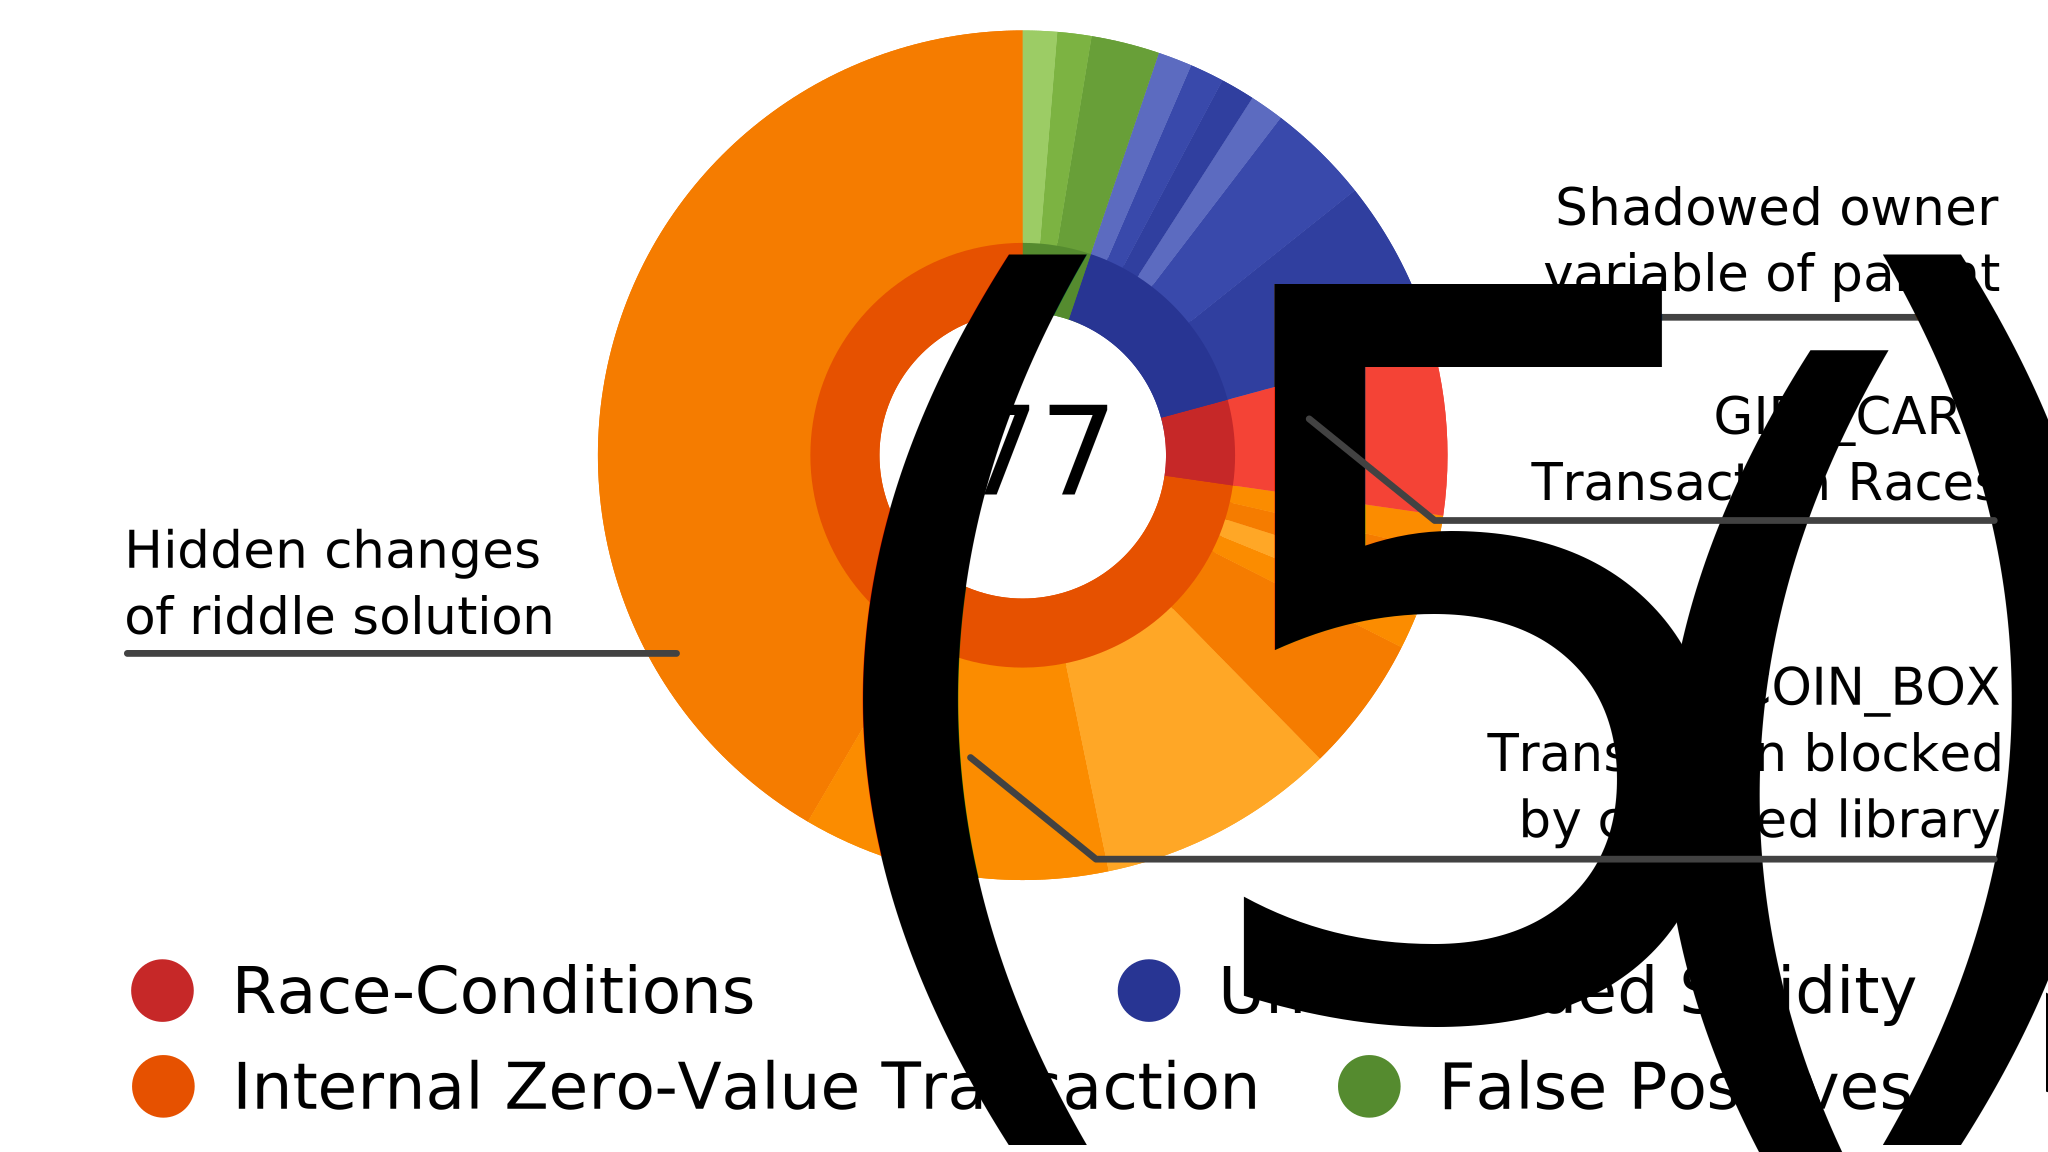
\includegraphics[width=12cm]{img/giftcard/analysis.pdf}
	\captionof{figure}[Amphicyon analysis of GIFT_CARD]{Analysis of the \texttt{GIFT_CARD}-contract using Amphicyon.}
	\label{figure:appendix:giftcard:amphicyon}
\end{minipage}

While manually categorizing the flagged contracts, the author first wrongly assumed this contract to be a false positive, because no internal zero-value transactions could be found on alternative blockchain explorers and there was no trace of underhanded Solidity code. The only way to recognize this type of honeypot is after it has latched -- which in this case had already happened leaving behind the suspicious two almost identical transactions at the same block height with a very different gas prices.

\pagebreak{}
